% \glsresetall
\chapter{Web Components} % Main chapter title
\label{Chapter4}

\lhead{Chapter 4. \emph{Web Components}}

Another option to address the issue of redundancies are WCs. Consisting of the following four standards, they provide reusable elements encapsulated in HTML tags.\cite{mdn_web_docs}

\begin{itemize}[noitemsep]
	\item Custom Elements
	\item Shadow DOM
	\item HTML Template
	\item ES Modules
\end{itemize}

The following sections will introduce the four standards of WCs with their functions and showcase what purpose they can serve for the context of this thesis.

\section{Custom Elements}

This standard of WCs provides an API via which new HTML tags can be defined and registered by the \texttt{CustomElementRegistry}. Since a single tag name can only be registered once, multiple registrations of the same element would lead to an exception, thereby making already registered tags reusable for the whole micro frontend landscape without reloading the code of the registered element.\cite{google_reusable_wcs}

\begin{figure}[!h]
	\centering
	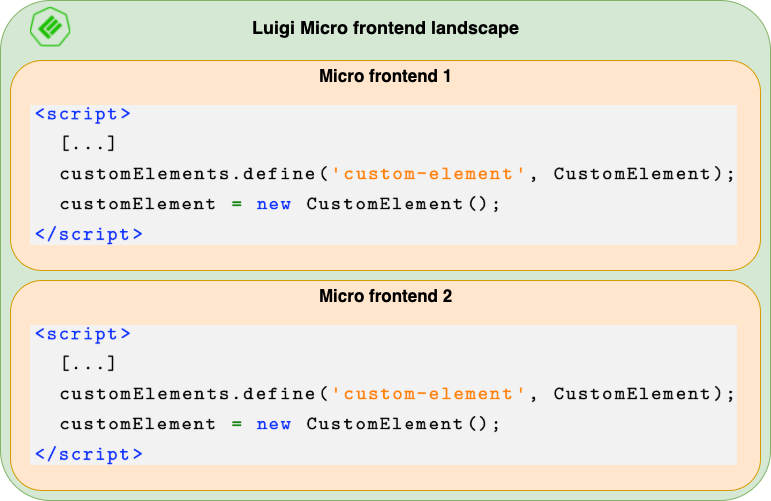
\includegraphics[width=0.8\textwidth]{Figures/customElements_registered_2.drawio.png}
	\caption{Simple micro frontend landscape using Web Components}
	\label{fig:same_wc_example}
\end{figure}

Figure \ref{fig:same_wc_example} shows a simple micro frontend landscape with Luigi using WCs. As displayed, both micro frontends are registering the same tag name \texttt{custom-element} using the \texttt{customElements} object. This object is a read-only property of the \texttt{Window} interface.
The scenario shown will cause a  \texttt{DOMException}, making it impossible to register the same tag twice.

The registration of WCs follows the \textit{"first come, first serve"} principle: The first micro frontend to register a tag name defines this tag and cannot be overwritten without reloading the page \cite{mdn_web_docs_define}.
Therefore, this standard is crucial for avoiding redundancies in micro frontend landscapes, by making it impossible to register same components with the same tag name.

\section{Shadow DOM}

The DOM (Document Object Model) represents the elements of a markup document in a tree-like structure, consisting of connected nodes. The commonly used markup language for websites is HTML  \cite{wc_shadow_dom}.
The Shadow DOM is also a DOM, but is attached to the actual DOM of the document. Underneath it, elements can be defined in the same way as they are in the regular DOM. The difference becomes apparent during the rendering of the document, when a page is loaded. The Shadow DOM elements are rendered separately from the DOM it is attached to.\cite{simon_thesis}

To understand the relationship between the two connected DOMs, the following terms have to be explained.

\begin{description}
	\item[Shadow host:] The attachment of the Shadow DOM to the normal DOM happens via a node inside the normal DOM.
	\item[Shadow tree:] Since the Shadow DOM is a DOM in itself, it consists of nodes in a tree-like structure.
	\item[Shadow boundary:] The Shadow DOM capsules its Shadow tree and renders it separately from the actual DOM. This encapsulated area defines where the Shadow DOM begins and ends.
	\item[Shadow root:] Just like a regular DOM, a Shadow DOM has a root from where it originates.
\end{description}

\newpage
Figure \ref{fig:shadow_dom} visualizes the relations between the newly introduced terms.

\begin{figure}[!h]
	\centering
	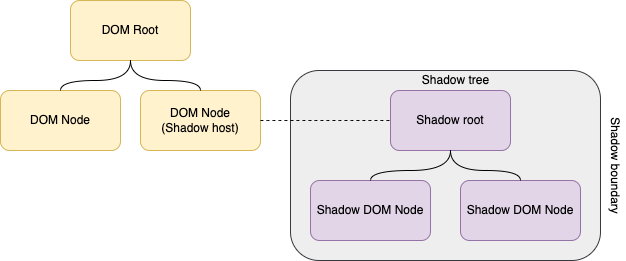
\includegraphics[width=1\textwidth]{Figures/shadow_dom.drawio.png}
	\caption{Shadow DOM architecture}
	\label{fig:shadow_dom}
\end{figure}

Through the isolation of the Shadow DOM's code, this standard offers a way to provide scoped HTML and CSS code to custom elements. As mentioned before, the nodes of the Shadow DOM are rendered separately. Therefore, styles, ids, names or even CSS classes and other configurations applied to a tag inside the Shadow DOM are not applied to the actual DOM.

The Shadow DOM, even though separated from the DOM, has an attribute via which it can be made accessible. By adding the \texttt{mode} attribute to the \texttt{this.attachShadow()} method, the visibility of the Shadow DOM to the document can be defined \cite{simon_thesis}. Possible values for the \texttt{mode} property are:

\begin{itemize}[noitemsep]
	\item \textbf{open}
	\item \textbf{closed}
\end{itemize}

This behavior is not meant to be used as a measure of security, since it can be overwritten. The Shadow DOM encapsulates every part of its DOM elements, that means HTML, CSS and JavaScript. The \texttt{document} object, available during runtime, remains the same for the regular DOM and for the Shadow DOM, though. Therefore, each configuration done in the Shadow DOM via scripts can be easily overwritten from any other script in the document, thus the mode can be changed even if initially set to \texttt{closed} \cite{shadow_dom_encapsulation}. For WCs, in particular, it is not recommended to use this mode at all, since it would make them less flexible for end users \cite{wc_shadow_dom_google}.

For the context of this thesis, the Shadow DOM standard offers means to individualize the registered WCs of a landscape. It can be used to apply customizations or add individual event listeners to specific components. This comes with a trade-off, though. The level of isolation increases through the encapsulation of code elements between the single components. This increase makes it difficult to guarantee that e.g. the same CSS class is not rendered in multiple different Shadow DOMs. Even though the redundancies would occur on code level and not on dependency level, they are redundancies nonetheless.

\section{HTML Template}

This standard offers a way to define reusable markup code. As a part of the HTML standard itself, the \texttt{template} tag is used to define templates. These are not rendered unless used by another element. The \texttt{slot} standard, serves a similar purpose as the \texttt{template} standard, but in a different way. Templates are defined HTML code snippets which can be cloned and inserted in other document elements or even elements rendered in the Shadow DOM.
Slots, on the other hand, serve as placeholder for either default markup texts or other DOM elements. Therefore, a template is a rather static piece of reusable HTML code, compared to slots.
Slots themselves are identified by their name, the content is inserted when the slot is addressed by its name.
Listings \ref{list:template_example} and \ref{list:slot_example} provide examples how exactly these two standards are used. \cite{wc_html_template_slots}

\begin{lstlisting}[language=HTML5,caption=Definition and usage of the \texttt{template} standard \cite{wc_html_template_slots}, label=list:template_example,  xleftmargin=.0\textwidth, xrightmargin=.0\textwidth]
<!-- Definition of the template -->
<template id="my-paragraph">
	<p>My paragraph</p>
</template>

<!-- Usage of the template in an Web Component -->
customElements.define('my-paragraph',
class extends HTMLElement {
	constructor() {
		super();
		let template = document.getElementById('my-paragraph');
		let templateContent = template.content;
		
		const shadowRoot = this.attachShadow({mode: 'open'})
		.appendChild(templateContent.cloneNode(true));
	}
});
\end{lstlisting}

It is important to note that the defined template in the listing is not rendered unless somehow included in a DOM (either Shadow DOM or the regular DOM), via JavaScript.

\newpage

\begin{lstlisting}[language=HTML5, caption=Definition and usage of the \texttt{slot} standard \cite{wc_html_template_slots}, label=list:slot_example,  xleftmargin=.0\textwidth, xrightmargin=.0\textwidth]
<!-- Definition of the slot -->
<p>
	<slot name="my-text">Default input</slot>
</p>

<!-- Usage of the slot in the markup document -->
<my-paragraph>
	<ul slot="my-text">
		<li>Some different input</li>
		<li>In a list!</li>
	</ul>
</my-paragraph>
\end{lstlisting}

As it can be seen in listing \ref{list:slot_example}, the \texttt{slot} definition has some default content defined. In the above case it is a simple text. When the slot is used, this content is overwritten by the content in the element which is calling the \texttt{slot} by its name.
In that case, the content is replaced by some list items.
Other than the templates, slots are always rendered if included in the markup via their respective names. The rendering of the content depends on whether the default content is overwritten or not.

Even though slots are an HTML standard, just as templates, their support for browsers is not always guaranteed. This is due to the fact that compared to templates, it is a rather new standard.

In combination, these two standards offer a way to define flexible, reusable markup code for WCs.\cite{wc_html_template_slots} 

When developing new WCs for a micro frontend landscape, this aspect can be used to reduce repetitive HTML code elements by serving them a template. Similar to the Shadow DOM, this feature could be used to apply more flexibility to the WCs by adding placeholders for customization. But, contrary to the Shadow DOM, this does not increase the level of isolation, since the rendered elements are not separated from the actual DOM. Redundant code snippets can be defined as reusable templates, thereby reducing the redundancies in the code itself.

\section{ES Modules}

The last standard is not referred to by every source, but according to \cite{wc_specifications}, it is a stable part of the WCs standard, via which JavaScript modules can be defined and reused by other documents.
Thus the development of WCs can be done in a modular way, making every component available to other documents, using the \texttt{type="module"} attribute.

\begin{lstlisting}[language=HTML5, caption=Importing modular Java Script documents into another \cite{wc_specifications}, label=list:es_modules_example,  xleftmargin=.0\textwidth, xrightmargin=.0\textwidth]
<!-- Import of the JS Module -->
<script type="module" src="awesome-explosion.js"></script>
	[...]
<script type="module">
	import 'awesome-explosion.js';
	[...]
	import {awesomeExplosion} from '@awesome-things/awesome-explosion';
</script>

<!-- Usage of the newly imported module -->
<awesome-explosion>
	[...]
</awesome-explosion>
\end{lstlisting}

Listing \ref{list:es_modules_example} shows such an import. Assuming the \texttt{awesome-explosion.js} files contains the definition of an element called \texttt{awesome-explosion}, these lines enable the document to use this element.\cite{wc_specifications}

This feature is essential for the developed prototype, since via this aspect the components are made available to the landscape. The used WCs are served as ES Modules to the landscape and are imported similarly as shown in \ref{list:es_modules_example}. Therefore, this aspect enables a component to be imported in multiple micro frontends as a module.

\section{Additional considerations}

There is a niche case which can be raised as an objection, concerning the WC technology. Since the registration and, therefore, the naming of elements is up to the developers, it can occur that two components are registered under the same tag name, but the elements themselves are different. In this case, it is up to the developers to use the standard properly.

Assuming a common micro frontend landscape where every micro frontend is developed by independent, isolated teams, using heterogenic frameworks, the mentioned issue might occur. Two teams use WCs and try to register different elements under the same tag name in the same landscape. This requires organizational interference on team level.

One way would be to define a namespace for every team when creating WCs e.g. Team 1 has the namespace \texttt{team-1}, causing a WC registered by the micro frontend of Team 1 to be named \texttt{team-1-tagname}. This could lead to redundancies, because there is no way of assuring that the \texttt{team-1-tagname} and \texttt{team-2-tagname} WCs are not the same.\cite{wc_best_practices}

A better way might be to assign a common WCs library like \textbf{UI5 Web Components} \cite{ui5_wc_github}. That way, the registered elements are provided by the library and are limited to a set of unique registrable tags. If another micro frontend would try and register an already registered element of the library, a warning is thrown but no error occurs.

Most WC libraries also offer so-called scoping options. This feature is employed when versions of the used components differ between micro frontends. It enables the developers to customize their WCs and register them under different tags. With this feature, it is made possible to register components according to their respective versions, by adding a version-specific suffix. That, of course, might lead to redundancies again. But it also reduces the dependency of the developer teams to always use the latest version of the component library or the first registered element in the landscape. \cite{ui5_webcomponents_scoping} \cite{openwc_scoping}



